% Gemini theme
% https://github.com/anishathalye/gemini

\documentclass[final,20pt]{beamer}

% ====================
% Packages
% ====================

\usepackage[ngerman]{babel}
\usepackage[T1]{fontenc}
\usepackage{lmodern}
\usepackage[size=a1,orientation=portrait,scale=1.4]{beamerposter}
\usetheme{gemini}
\usecolortheme{gemini}
\usepackage{graphicx}
\usepackage{tikz}
\usepackage{pgfplots}
\usepackage{svg}

% ====================
% Lengths
% ====================

% If you have N columns, choose \sepwidth and \colwidth such that
% (N+1)*\sepwidth + N*\colwidth = \paperwidth
\newlength{\sepwidth}
\newlength{\colwidth}
\setlength{\sepwidth}{0.02\paperwidth}
\setlength{\colwidth}{0.47\paperwidth}

\newcommand{\separatorcolumn}{\begin{column}{\sepwidth}\end{column}}
\addto\extrasngerman{\def\figureautorefname{Abb.}}

\addtobeamertemplate{headline}{} 
{
	\begin{tikzpicture}[remember picture, overlay]
	\node [anchor=north east, inner sep=4cm]  at (current page.north east)
	{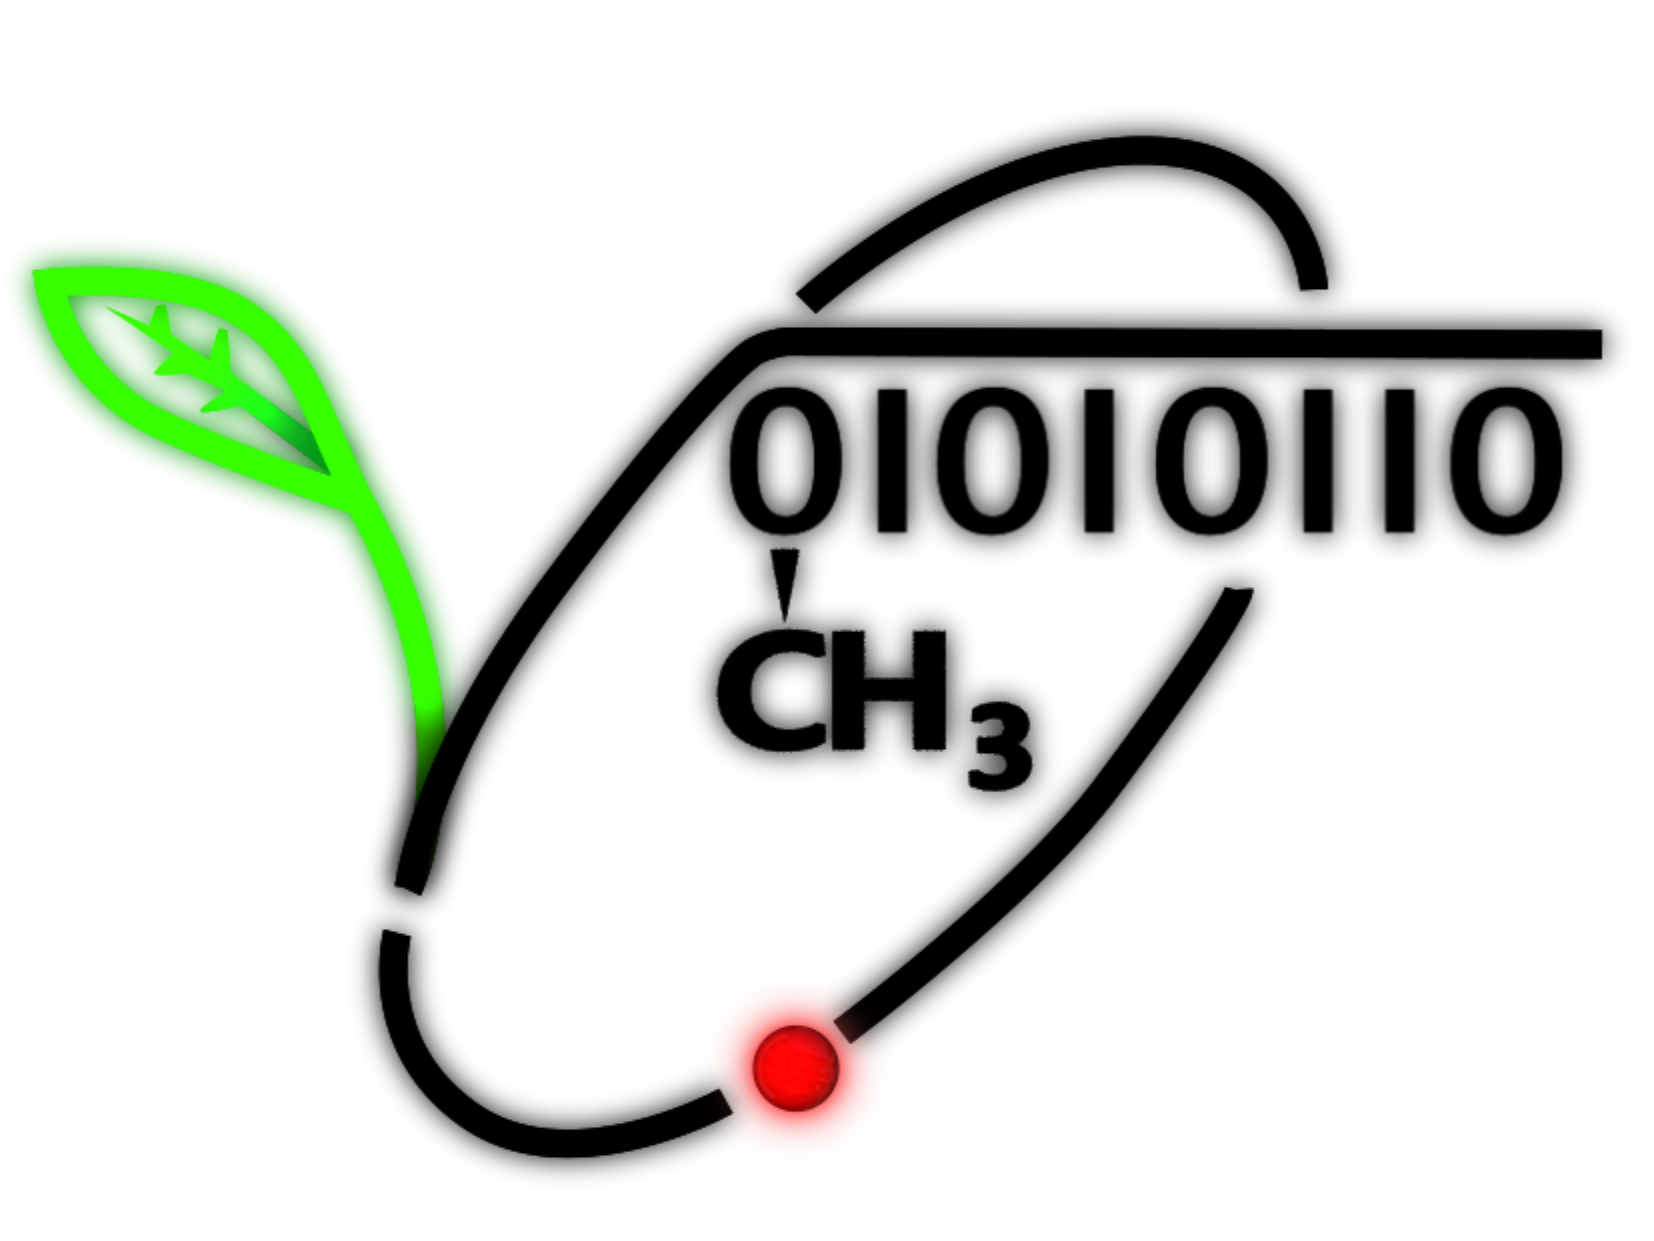
\includegraphics[height=5cm]{pics/logo}};
	\end{tikzpicture}}
% ====================
% Title
% ====================

\title{Apoplexy - Ein Fitnesstracker zur Rehabilitation von Schlaganfall-Patienten}

\author{Lukas Rost}
\institute{Albert-Schweitzer-Gymnasium Erfurt}

% ====================
% Body
% ====================

\begin{document}

\begin{frame}[t]
\begin{columns}[t]
\separatorcolumn

\begin{column}{\colwidth}

  \begin{alertblock}{Schlaganfall als Krankheitsbild}
  	\begin{itemize}
  		\item plötzliche Durchblutungsstörung im Gehirn
  		\item regionaler Mangel an Sauerstoff und Nährstoffen
  		\item Absterben von Gehirngewebe
  	\end{itemize}
  \begin{figure}[H]
  	\centering
  	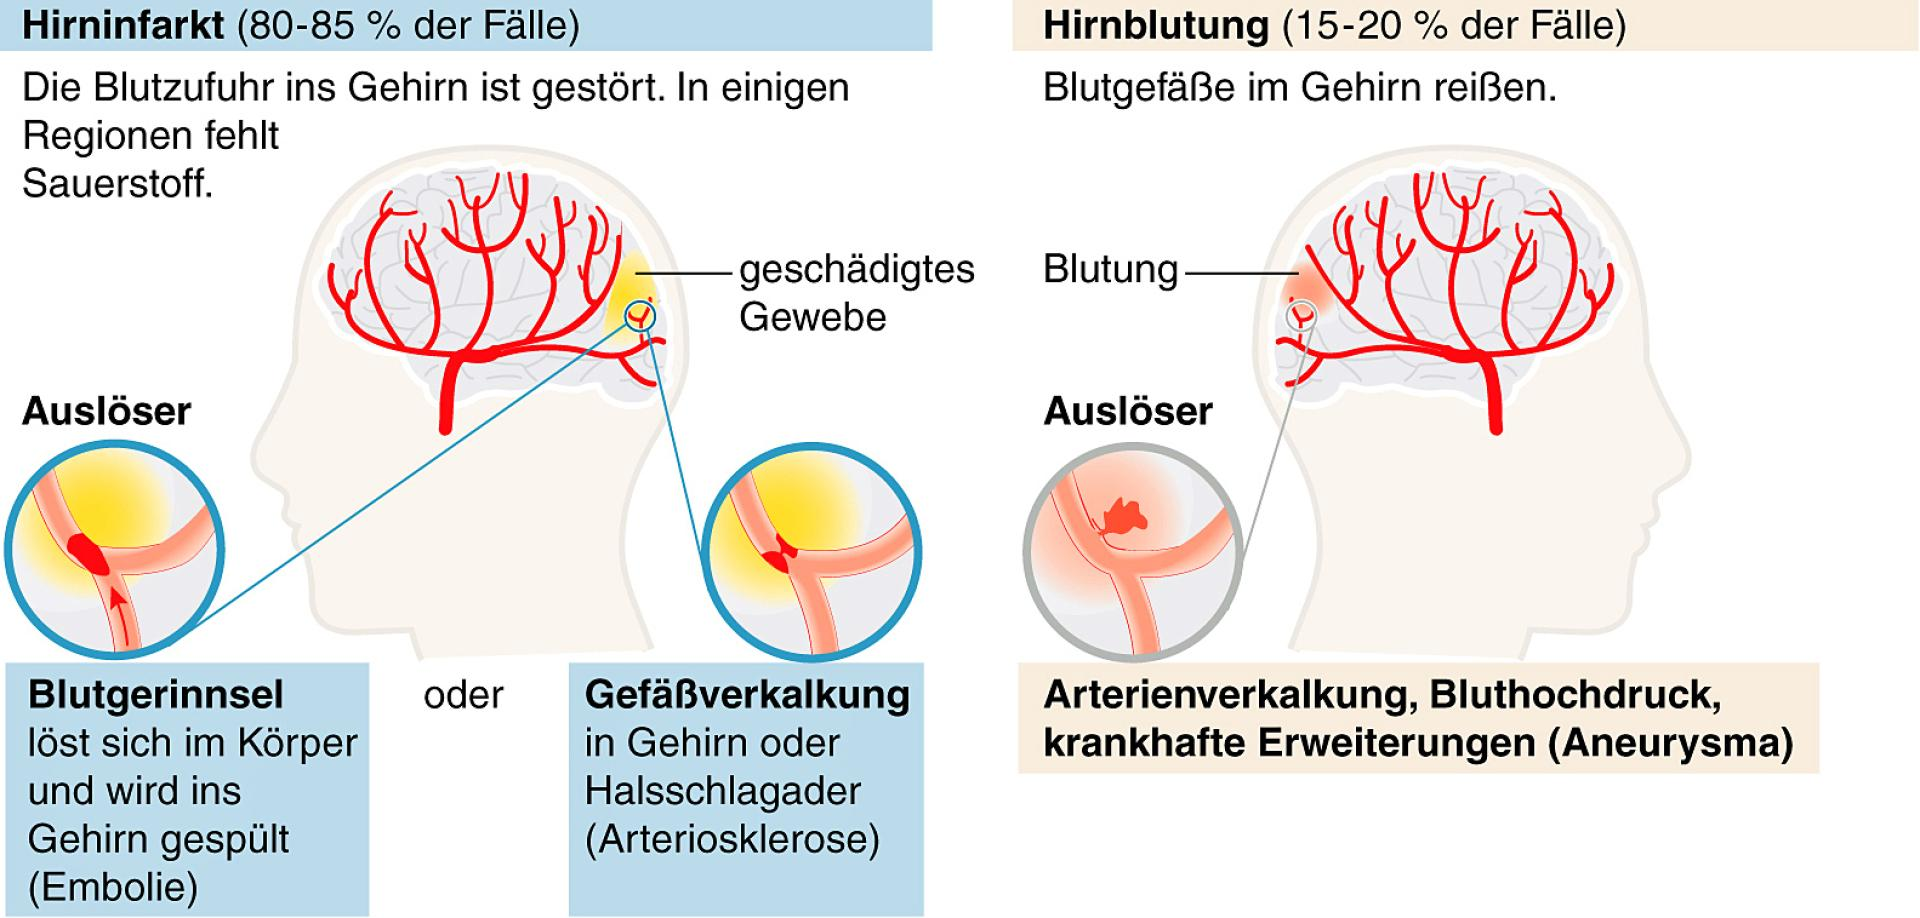
\includegraphics[width=0.8\colwidth]{pics/sentst}
  	\caption{Arten des Schlaganfalls}
  \end{figure}  
  	\begin{figure}[H]
  		\centering
  		\includesvg[width=0.8\colwidth]{pics/Schlaganfall}
  		\caption{Erkennung durch den FAST-Test}
  	\end{figure}

  \end{alertblock}

  \begin{alertblock}{Therapiemethoden und Bewegungsübungen}

    \begin{figure}[H]
    	\centering
    	\includesvg[width=0.8\colwidth]{pics/therapie}
    \end{figure}

	\begin{figure}[H]
		\centering
		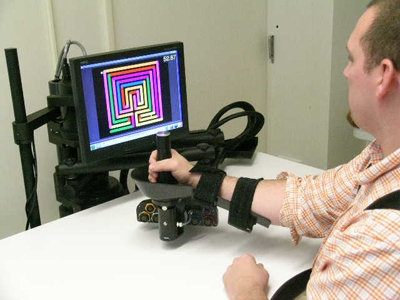
\includegraphics[width=0.5\colwidth]{pics/armrobot}
		\caption{Ein Gerät nach dem Armrobot-Prinzip}
		\label{fig:armrobot}
	\end{figure}

  \end{alertblock}

\end{column}

\separatorcolumn

\begin{column}{\colwidth}  
	
	\begin{alertblock}{Problemstellung}
		\begin{itemize}
			\item Unterstützung der \textbf{Therapie} einer durch Schlaganfall entstandenen \textbf{Armlähmung} mittels eines zu entwickelnden Geräts
			\item Messung der Kontraktion der Armmuskeln per \textbf{Elektromyographie} und Übertragung an ein Smartphone mit Begleitapp
			\item \textbf{Motivationsfunktion} für Patienten mittels \textbf{Gamification-Prinzip} (Erfahrungspunkte, Badges und Quests)
			\item Durchführung von \textbf{Übungen}, \textbf{Minispiel}, Erinnerung an Übungen
			\item Ansätze zur Einbindung in eine medizinisch anerkannte \textbf{Therapiemethode} (Unterstützung für schädigungsorientiertes Training)
		\end{itemize}
	\end{alertblock}
  
  \begin{alertblock}{Motivation durch Gamification}
  	\begin{itemize}
  		\item \textbf{Definition:} Verwendung von spieltypischen Mechaniken außerhalb reiner Spiele, mit dem Ziel, das Verhalten von Menschen zu beeinflussen \begin{small}(Breuer)\end{small}
  		\item \textbf{Ziel:} Steigerung der Nutzungsmotivation
  		\item \textbf{Ausnutzung} des menschlichen Spieltriebs:
  		\begin{itemize}
  			\item positive Anreize zur Anregung zu einem bestimmten Verhalten
  			\item negative Anreize wollen vom Nutzer vermieden werden
  		\end{itemize}  		
  	\end{itemize}
  \begin{figure}[H]
  	\centering
  	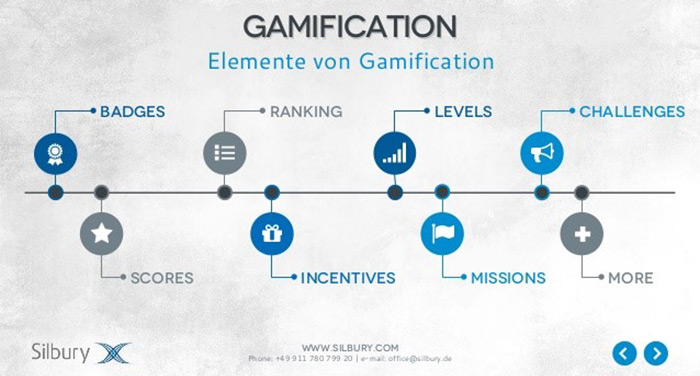
\includegraphics[width=0.65\colwidth]{pics/elements}
  	\caption{Einsatz spieltypischer Mechanismen}
  \end{figure}
  	\begin{figure}[H]
  		\centering
  		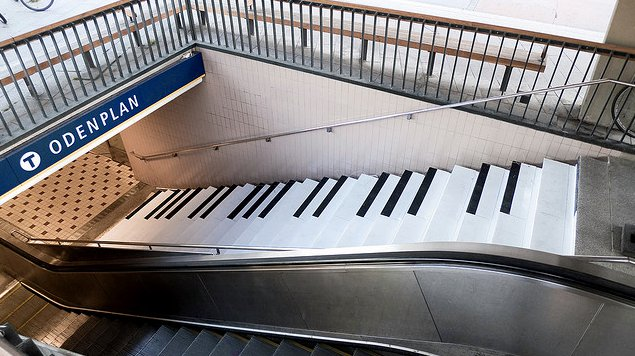
\includegraphics[width=0.65\colwidth]{pics/pianostairs}
  		\caption{ \centering Die Klaviertreppe aus dem Projekt The Fun Theory als Beispiel für gelungene Gamification}
  	\end{figure}
  \end{alertblock}

  \begin{alertblock}{Rückkopplung durch Biofeedback}
  	\begin{itemize}
  		\item \textbf{Körperfunktionen} und biologische Vorgänge sind der Sinneswahrnehmung normalerweise nicht zugänglich
  		\item können jedoch mit \textbf{elektronischen Hilfsmitteln} beobachtbar gemacht werden
  		\item \textbf{Rückkopplung:} Patient kann Kontrolle über die Körperfunktion ausüben
  	\end{itemize}

    \begin{figure}
      \centering
      \begin{tikzpicture}
        \begin{axis}[
            scale only axis,
            no markers,
            domain=0:2*pi,
            samples=100,
            axis lines=center,
            axis line style={-},
            ticks=none]
          \addplot[red] {sin(deg(x))};
          \addplot[blue] {cos(deg(x))};
        \end{axis}
      \end{tikzpicture}
      \caption{mögliche Visualisierung aufgezeichneter Messwerte}
    \end{figure}

  \end{alertblock}

\end{column}

\separatorcolumn
\end{columns}
\end{frame}

\end{document}
